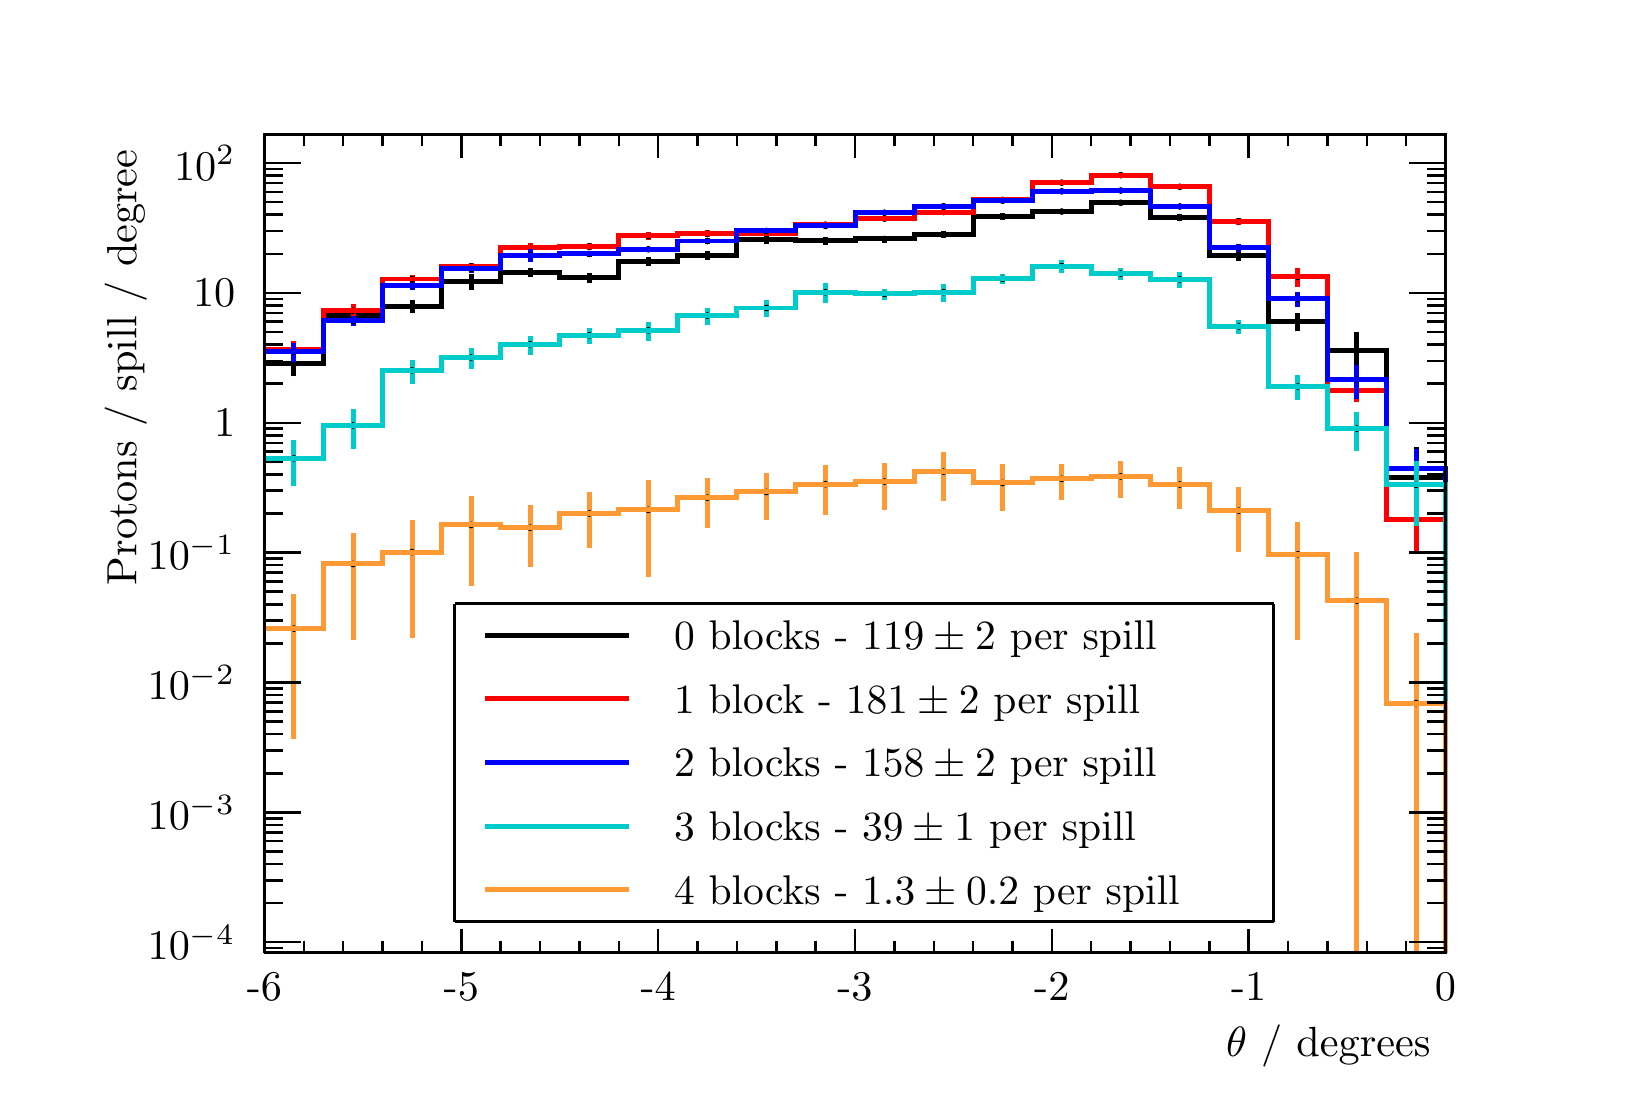
\begin{tikzpicture}
\pgfdeclareplotmark{cross} {
\pgfpathmoveto{\pgfpoint{-0.3\pgfplotmarksize}{\pgfplotmarksize}}
\pgfpathlineto{\pgfpoint{+0.3\pgfplotmarksize}{\pgfplotmarksize}}
\pgfpathlineto{\pgfpoint{+0.3\pgfplotmarksize}{0.3\pgfplotmarksize}}
\pgfpathlineto{\pgfpoint{+1\pgfplotmarksize}{0.3\pgfplotmarksize}}
\pgfpathlineto{\pgfpoint{+1\pgfplotmarksize}{-0.3\pgfplotmarksize}}
\pgfpathlineto{\pgfpoint{+0.3\pgfplotmarksize}{-0.3\pgfplotmarksize}}
\pgfpathlineto{\pgfpoint{+0.3\pgfplotmarksize}{-1.\pgfplotmarksize}}
\pgfpathlineto{\pgfpoint{-0.3\pgfplotmarksize}{-1.\pgfplotmarksize}}
\pgfpathlineto{\pgfpoint{-0.3\pgfplotmarksize}{-0.3\pgfplotmarksize}}
\pgfpathlineto{\pgfpoint{-1.\pgfplotmarksize}{-0.3\pgfplotmarksize}}
\pgfpathlineto{\pgfpoint{-1.\pgfplotmarksize}{0.3\pgfplotmarksize}}
\pgfpathlineto{\pgfpoint{-0.3\pgfplotmarksize}{0.3\pgfplotmarksize}}
\pgfpathclose
\pgfusepathqstroke
}
\pgfdeclareplotmark{cross*} {
\pgfpathmoveto{\pgfpoint{-0.3\pgfplotmarksize}{\pgfplotmarksize}}
\pgfpathlineto{\pgfpoint{+0.3\pgfplotmarksize}{\pgfplotmarksize}}
\pgfpathlineto{\pgfpoint{+0.3\pgfplotmarksize}{0.3\pgfplotmarksize}}
\pgfpathlineto{\pgfpoint{+1\pgfplotmarksize}{0.3\pgfplotmarksize}}
\pgfpathlineto{\pgfpoint{+1\pgfplotmarksize}{-0.3\pgfplotmarksize}}
\pgfpathlineto{\pgfpoint{+0.3\pgfplotmarksize}{-0.3\pgfplotmarksize}}
\pgfpathlineto{\pgfpoint{+0.3\pgfplotmarksize}{-1.\pgfplotmarksize}}
\pgfpathlineto{\pgfpoint{-0.3\pgfplotmarksize}{-1.\pgfplotmarksize}}
\pgfpathlineto{\pgfpoint{-0.3\pgfplotmarksize}{-0.3\pgfplotmarksize}}
\pgfpathlineto{\pgfpoint{-1.\pgfplotmarksize}{-0.3\pgfplotmarksize}}
\pgfpathlineto{\pgfpoint{-1.\pgfplotmarksize}{0.3\pgfplotmarksize}}
\pgfpathlineto{\pgfpoint{-0.3\pgfplotmarksize}{0.3\pgfplotmarksize}}
\pgfpathclose
\pgfusepathqfillstroke
}
\pgfdeclareplotmark{newstar} {
\pgfpathmoveto{\pgfqpoint{0pt}{\pgfplotmarksize}}
\pgfpathlineto{\pgfqpointpolar{44}{0.5\pgfplotmarksize}}
\pgfpathlineto{\pgfqpointpolar{18}{\pgfplotmarksize}}
\pgfpathlineto{\pgfqpointpolar{-20}{0.5\pgfplotmarksize}}
\pgfpathlineto{\pgfqpointpolar{-54}{\pgfplotmarksize}}
\pgfpathlineto{\pgfqpointpolar{-90}{0.5\pgfplotmarksize}}
\pgfpathlineto{\pgfqpointpolar{234}{\pgfplotmarksize}}
\pgfpathlineto{\pgfqpointpolar{198}{0.5\pgfplotmarksize}}
\pgfpathlineto{\pgfqpointpolar{162}{\pgfplotmarksize}}
\pgfpathlineto{\pgfqpointpolar{134}{0.5\pgfplotmarksize}}
\pgfpathclose
\pgfusepathqstroke
}
\pgfdeclareplotmark{newstar*} {
\pgfpathmoveto{\pgfqpoint{0pt}{\pgfplotmarksize}}
\pgfpathlineto{\pgfqpointpolar{44}{0.5\pgfplotmarksize}}
\pgfpathlineto{\pgfqpointpolar{18}{\pgfplotmarksize}}
\pgfpathlineto{\pgfqpointpolar{-20}{0.5\pgfplotmarksize}}
\pgfpathlineto{\pgfqpointpolar{-54}{\pgfplotmarksize}}
\pgfpathlineto{\pgfqpointpolar{-90}{0.5\pgfplotmarksize}}
\pgfpathlineto{\pgfqpointpolar{234}{\pgfplotmarksize}}
\pgfpathlineto{\pgfqpointpolar{198}{0.5\pgfplotmarksize}}
\pgfpathlineto{\pgfqpointpolar{162}{\pgfplotmarksize}}
\pgfpathlineto{\pgfqpointpolar{134}{0.5\pgfplotmarksize}}
\pgfpathclose
\pgfusepathqfillstroke
}
\definecolor{c}{rgb}{1,1,1};
\draw [color=c, fill=c] (0,0) rectangle (20,13.4957);
\draw [color=c, fill=c] (3,1.75444) rectangle (18,12.1461);
\definecolor{c}{rgb}{0,0,0};
\draw [c,line width=0.9] (3,1.75444) -- (3,12.1461) -- (18,12.1461) -- (18,1.75444) -- (3,1.75444);
\definecolor{c}{rgb}{1,1,1};
\draw [color=c, fill=c] (3,1.75444) rectangle (18,12.1461);
\definecolor{c}{rgb}{0,0,0};
\draw [c,line width=0.9] (3,1.75444) -- (3,12.1461) -- (18,12.1461) -- (18,1.75444) -- (3,1.75444);
\draw [c,line width=0.9] (3,1.75444) -- (3.75,1.75444) -- (3.75,1.75444) -- (4.5,1.75444) -- (4.5,1.75444) -- (5.25,1.75444) -- (5.25,1.75444) -- (6,1.75444) -- (6,1.75444) -- (6.75,1.75444) -- (6.75,1.75444) -- (7.5,1.75444) -- (7.5,1.75444) --
 (8.25,1.75444) -- (8.25,1.75444) -- (9,1.75444) -- (9,1.75444) -- (9.75,1.75444) -- (9.75,1.75444) -- (10.5,1.75444) -- (10.5,1.75444) -- (11.25,1.75444) -- (11.25,1.75444) -- (12,1.75444) -- (12,1.75444) -- (12.75,1.75444) -- (12.75,1.75444) --
 (13.5,1.75444) -- (13.5,1.75444) -- (14.25,1.75444) -- (14.25,1.75444) -- (15,1.75444) -- (15,1.75444) -- (15.75,1.75444) -- (15.75,1.75444) -- (16.5,1.75444) -- (16.5,1.75444) -- (17.25,1.75444) -- (17.25,1.75444) -- (18,1.75444) -- (18,1.75444);
\draw [c,line width=0.9] (3,1.75444) -- (18,1.75444);
\draw [c,line width=0.9] (3,2.05809) -- (3,1.75444);
\draw [c,line width=0.9] (3.5,1.90627) -- (3.5,1.75444);
\draw [c,line width=0.9] (4,1.90627) -- (4,1.75444);
\draw [c,line width=0.9] (4.5,1.90627) -- (4.5,1.75444);
\draw [c,line width=0.9] (5,1.90627) -- (5,1.75444);
\draw [c,line width=0.9] (5.5,2.05809) -- (5.5,1.75444);
\draw [c,line width=0.9] (6,1.90627) -- (6,1.75444);
\draw [c,line width=0.9] (6.5,1.90627) -- (6.5,1.75444);
\draw [c,line width=0.9] (7,1.90627) -- (7,1.75444);
\draw [c,line width=0.9] (7.5,1.90627) -- (7.5,1.75444);
\draw [c,line width=0.9] (8,2.05809) -- (8,1.75444);
\draw [c,line width=0.9] (8.5,1.90627) -- (8.5,1.75444);
\draw [c,line width=0.9] (9,1.90627) -- (9,1.75444);
\draw [c,line width=0.9] (9.5,1.90627) -- (9.5,1.75444);
\draw [c,line width=0.9] (10,1.90627) -- (10,1.75444);
\draw [c,line width=0.9] (10.5,2.05809) -- (10.5,1.75444);
\draw [c,line width=0.9] (11,1.90627) -- (11,1.75444);
\draw [c,line width=0.9] (11.5,1.90627) -- (11.5,1.75444);
\draw [c,line width=0.9] (12,1.90627) -- (12,1.75444);
\draw [c,line width=0.9] (12.5,1.90627) -- (12.5,1.75444);
\draw [c,line width=0.9] (13,2.05809) -- (13,1.75444);
\draw [c,line width=0.9] (13.5,1.90627) -- (13.5,1.75444);
\draw [c,line width=0.9] (14,1.90627) -- (14,1.75444);
\draw [c,line width=0.9] (14.5,1.90627) -- (14.5,1.75444);
\draw [c,line width=0.9] (15,1.90627) -- (15,1.75444);
\draw [c,line width=0.9] (15.5,2.05809) -- (15.5,1.75444);
\draw [c,line width=0.9] (16,1.90627) -- (16,1.75444);
\draw [c,line width=0.9] (16.5,1.90627) -- (16.5,1.75444);
\draw [c,line width=0.9] (17,1.90627) -- (17,1.75444);
\draw [c,line width=0.9] (17.5,1.90627) -- (17.5,1.75444);
\draw [c,line width=0.9] (18,2.05809) -- (18,1.75444);
\draw [anchor=base] (3,1.14713) node[scale=1.52731, color=c, rotate=0]{-6};
\draw [anchor=base] (5.5,1.14713) node[scale=1.52731, color=c, rotate=0]{-5};
\draw [anchor=base] (8,1.14713) node[scale=1.52731, color=c, rotate=0]{-4};
\draw [anchor=base] (10.5,1.14713) node[scale=1.52731, color=c, rotate=0]{-3};
\draw [anchor=base] (13,1.14713) node[scale=1.52731, color=c, rotate=0]{-2};
\draw [anchor=base] (15.5,1.14713) node[scale=1.52731, color=c, rotate=0]{-1};
\draw [anchor=base] (18,1.14713) node[scale=1.52731, color=c, rotate=0]{0};
\draw [anchor= east] (18,0.566819) node[scale=1.52731, color=c, rotate=0]{$ \theta$ / degrees};
\draw [c,line width=0.9] (3,12.1461) -- (18,12.1461);
\draw [c,line width=0.9] (3,11.8425) -- (3,12.1461);
\draw [c,line width=0.9] (3.5,11.9943) -- (3.5,12.1461);
\draw [c,line width=0.9] (4,11.9943) -- (4,12.1461);
\draw [c,line width=0.9] (4.5,11.9943) -- (4.5,12.1461);
\draw [c,line width=0.9] (5,11.9943) -- (5,12.1461);
\draw [c,line width=0.9] (5.5,11.8425) -- (5.5,12.1461);
\draw [c,line width=0.9] (6,11.9943) -- (6,12.1461);
\draw [c,line width=0.9] (6.5,11.9943) -- (6.5,12.1461);
\draw [c,line width=0.9] (7,11.9943) -- (7,12.1461);
\draw [c,line width=0.9] (7.5,11.9943) -- (7.5,12.1461);
\draw [c,line width=0.9] (8,11.8425) -- (8,12.1461);
\draw [c,line width=0.9] (8.5,11.9943) -- (8.5,12.1461);
\draw [c,line width=0.9] (9,11.9943) -- (9,12.1461);
\draw [c,line width=0.9] (9.5,11.9943) -- (9.5,12.1461);
\draw [c,line width=0.9] (10,11.9943) -- (10,12.1461);
\draw [c,line width=0.9] (10.5,11.8425) -- (10.5,12.1461);
\draw [c,line width=0.9] (11,11.9943) -- (11,12.1461);
\draw [c,line width=0.9] (11.5,11.9943) -- (11.5,12.1461);
\draw [c,line width=0.9] (12,11.9943) -- (12,12.1461);
\draw [c,line width=0.9] (12.5,11.9943) -- (12.5,12.1461);
\draw [c,line width=0.9] (13,11.8425) -- (13,12.1461);
\draw [c,line width=0.9] (13.5,11.9943) -- (13.5,12.1461);
\draw [c,line width=0.9] (14,11.9943) -- (14,12.1461);
\draw [c,line width=0.9] (14.5,11.9943) -- (14.5,12.1461);
\draw [c,line width=0.9] (15,11.9943) -- (15,12.1461);
\draw [c,line width=0.9] (15.5,11.8425) -- (15.5,12.1461);
\draw [c,line width=0.9] (16,11.9943) -- (16,12.1461);
\draw [c,line width=0.9] (16.5,11.9943) -- (16.5,12.1461);
\draw [c,line width=0.9] (17,11.9943) -- (17,12.1461);
\draw [c,line width=0.9] (17.5,11.9943) -- (17.5,12.1461);
\draw [c,line width=0.9] (18,11.8425) -- (18,12.1461);
\draw [c,line width=0.9] (3,1.75444) -- (3,12.1461);
\draw [c,line width=0.9] (3.231,1.81225) -- (3,1.81225);
\draw [c,line width=0.9] (3.462,1.88772) -- (3,1.88772);
\draw [anchor= east] (2.82,1.88772) node[scale=1.52731, color=c, rotate=0]{$10^{-4}$};
\draw [c,line width=0.9] (3.231,2.38422) -- (3,2.38422);
\draw [c,line width=0.9] (3.231,2.67466) -- (3,2.67466);
\draw [c,line width=0.9] (3.231,2.88072) -- (3,2.88072);
\draw [c,line width=0.9] (3.231,3.04056) -- (3,3.04056);
\draw [c,line width=0.9] (3.231,3.17116) -- (3,3.17116);
\draw [c,line width=0.9] (3.231,3.28158) -- (3,3.28158);
\draw [c,line width=0.9] (3.231,3.37722) -- (3,3.37722);
\draw [c,line width=0.9] (3.231,3.46159) -- (3,3.46159);
\draw [c,line width=0.9] (3.462,3.53706) -- (3,3.53706);
\draw [anchor= east] (2.82,3.53706) node[scale=1.52731, color=c, rotate=0]{$10^{-3}$};
\draw [c,line width=0.9] (3.231,4.03357) -- (3,4.03357);
\draw [c,line width=0.9] (3.231,4.324) -- (3,4.324);
\draw [c,line width=0.9] (3.231,4.53007) -- (3,4.53007);
\draw [c,line width=0.9] (3.231,4.68991) -- (3,4.68991);
\draw [c,line width=0.9] (3.231,4.8205) -- (3,4.8205);
\draw [c,line width=0.9] (3.231,4.93092) -- (3,4.93092);
\draw [c,line width=0.9] (3.231,5.02657) -- (3,5.02657);
\draw [c,line width=0.9] (3.231,5.11094) -- (3,5.11094);
\draw [c,line width=0.9] (3.462,5.18641) -- (3,5.18641);
\draw [anchor= east] (2.82,5.18641) node[scale=1.52731, color=c, rotate=0]{$10^{-2}$};
\draw [c,line width=0.9] (3.231,5.68291) -- (3,5.68291);
\draw [c,line width=0.9] (3.231,5.97335) -- (3,5.97335);
\draw [c,line width=0.9] (3.231,6.17941) -- (3,6.17941);
\draw [c,line width=0.9] (3.231,6.33925) -- (3,6.33925);
\draw [c,line width=0.9] (3.231,6.46985) -- (3,6.46985);
\draw [c,line width=0.9] (3.231,6.58027) -- (3,6.58027);
\draw [c,line width=0.9] (3.231,6.67592) -- (3,6.67592);
\draw [c,line width=0.9] (3.231,6.76028) -- (3,6.76028);
\draw [c,line width=0.9] (3.462,6.83575) -- (3,6.83575);
\draw [anchor= east] (2.82,6.83575) node[scale=1.52731, color=c, rotate=0]{$10^{-1}$};
\draw [c,line width=0.9] (3.231,7.33226) -- (3,7.33226);
\draw [c,line width=0.9] (3.231,7.62269) -- (3,7.62269);
\draw [c,line width=0.9] (3.231,7.82876) -- (3,7.82876);
\draw [c,line width=0.9] (3.231,7.9886) -- (3,7.9886);
\draw [c,line width=0.9] (3.231,8.11919) -- (3,8.11919);
\draw [c,line width=0.9] (3.231,8.22961) -- (3,8.22961);
\draw [c,line width=0.9] (3.231,8.32526) -- (3,8.32526);
\draw [c,line width=0.9] (3.231,8.40963) -- (3,8.40963);
\draw [c,line width=0.9] (3.462,8.4851) -- (3,8.4851);
\draw [anchor= east] (2.82,8.4851) node[scale=1.52731, color=c, rotate=0]{1};
\draw [c,line width=0.9] (3.231,8.9816) -- (3,8.9816);
\draw [c,line width=0.9] (3.231,9.27204) -- (3,9.27204);
\draw [c,line width=0.9] (3.231,9.4781) -- (3,9.4781);
\draw [c,line width=0.9] (3.231,9.63794) -- (3,9.63794);
\draw [c,line width=0.9] (3.231,9.76854) -- (3,9.76854);
\draw [c,line width=0.9] (3.231,9.87896) -- (3,9.87896);
\draw [c,line width=0.9] (3.231,9.97461) -- (3,9.97461);
\draw [c,line width=0.9] (3.231,10.059) -- (3,10.059);
\draw [c,line width=0.9] (3.462,10.1344) -- (3,10.1344);
\draw [anchor= east] (2.82,10.1344) node[scale=1.52731, color=c, rotate=0]{10};
\draw [c,line width=0.9] (3.231,10.6309) -- (3,10.6309);
\draw [c,line width=0.9] (3.231,10.9214) -- (3,10.9214);
\draw [c,line width=0.9] (3.231,11.1274) -- (3,11.1274);
\draw [c,line width=0.9] (3.231,11.2873) -- (3,11.2873);
\draw [c,line width=0.9] (3.231,11.4179) -- (3,11.4179);
\draw [c,line width=0.9] (3.231,11.5283) -- (3,11.5283);
\draw [c,line width=0.9] (3.231,11.624) -- (3,11.624);
\draw [c,line width=0.9] (3.231,11.7083) -- (3,11.7083);
\draw [c,line width=0.9] (3.462,11.7838) -- (3,11.7838);
\draw [anchor= east] (2.82,11.7838) node[scale=1.52731, color=c, rotate=0]{$10^{2}$};
\draw [anchor= east] (1.24,12.1461) node[scale=1.52731, color=c, rotate=90]{ Protons / spill / degree};
\draw [c,line width=0.9] (18,1.75444) -- (18,12.1461);
\draw [c,line width=0.9] (17.769,1.81225) -- (18,1.81225);
\draw [c,line width=0.9] (17.538,1.88772) -- (18,1.88772);
\draw [c,line width=0.9] (17.769,2.38422) -- (18,2.38422);
\draw [c,line width=0.9] (17.769,2.67466) -- (18,2.67466);
\draw [c,line width=0.9] (17.769,2.88072) -- (18,2.88072);
\draw [c,line width=0.9] (17.769,3.04056) -- (18,3.04056);
\draw [c,line width=0.9] (17.769,3.17116) -- (18,3.17116);
\draw [c,line width=0.9] (17.769,3.28158) -- (18,3.28158);
\draw [c,line width=0.9] (17.769,3.37722) -- (18,3.37722);
\draw [c,line width=0.9] (17.769,3.46159) -- (18,3.46159);
\draw [c,line width=0.9] (17.538,3.53706) -- (18,3.53706);
\draw [c,line width=0.9] (17.769,4.03357) -- (18,4.03357);
\draw [c,line width=0.9] (17.769,4.324) -- (18,4.324);
\draw [c,line width=0.9] (17.769,4.53007) -- (18,4.53007);
\draw [c,line width=0.9] (17.769,4.68991) -- (18,4.68991);
\draw [c,line width=0.9] (17.769,4.8205) -- (18,4.8205);
\draw [c,line width=0.9] (17.769,4.93092) -- (18,4.93092);
\draw [c,line width=0.9] (17.769,5.02657) -- (18,5.02657);
\draw [c,line width=0.9] (17.769,5.11094) -- (18,5.11094);
\draw [c,line width=0.9] (17.538,5.18641) -- (18,5.18641);
\draw [c,line width=0.9] (17.769,5.68291) -- (18,5.68291);
\draw [c,line width=0.9] (17.769,5.97335) -- (18,5.97335);
\draw [c,line width=0.9] (17.769,6.17941) -- (18,6.17941);
\draw [c,line width=0.9] (17.769,6.33925) -- (18,6.33925);
\draw [c,line width=0.9] (17.769,6.46985) -- (18,6.46985);
\draw [c,line width=0.9] (17.769,6.58027) -- (18,6.58027);
\draw [c,line width=0.9] (17.769,6.67592) -- (18,6.67592);
\draw [c,line width=0.9] (17.769,6.76028) -- (18,6.76028);
\draw [c,line width=0.9] (17.538,6.83575) -- (18,6.83575);
\draw [c,line width=0.9] (17.769,7.33226) -- (18,7.33226);
\draw [c,line width=0.9] (17.769,7.62269) -- (18,7.62269);
\draw [c,line width=0.9] (17.769,7.82876) -- (18,7.82876);
\draw [c,line width=0.9] (17.769,7.9886) -- (18,7.9886);
\draw [c,line width=0.9] (17.769,8.11919) -- (18,8.11919);
\draw [c,line width=0.9] (17.769,8.22961) -- (18,8.22961);
\draw [c,line width=0.9] (17.769,8.32526) -- (18,8.32526);
\draw [c,line width=0.9] (17.769,8.40963) -- (18,8.40963);
\draw [c,line width=0.9] (17.538,8.4851) -- (18,8.4851);
\draw [c,line width=0.9] (17.769,8.9816) -- (18,8.9816);
\draw [c,line width=0.9] (17.769,9.27204) -- (18,9.27204);
\draw [c,line width=0.9] (17.769,9.4781) -- (18,9.4781);
\draw [c,line width=0.9] (17.769,9.63794) -- (18,9.63794);
\draw [c,line width=0.9] (17.769,9.76854) -- (18,9.76854);
\draw [c,line width=0.9] (17.769,9.87896) -- (18,9.87896);
\draw [c,line width=0.9] (17.769,9.97461) -- (18,9.97461);
\draw [c,line width=0.9] (17.769,10.059) -- (18,10.059);
\draw [c,line width=0.9] (17.538,10.1344) -- (18,10.1344);
\draw [c,line width=0.9] (17.769,10.6309) -- (18,10.6309);
\draw [c,line width=0.9] (17.769,10.9214) -- (18,10.9214);
\draw [c,line width=0.9] (17.769,11.1274) -- (18,11.1274);
\draw [c,line width=0.9] (17.769,11.2873) -- (18,11.2873);
\draw [c,line width=0.9] (17.769,11.4179) -- (18,11.4179);
\draw [c,line width=0.9] (17.769,11.5283) -- (18,11.5283);
\draw [c,line width=0.9] (17.769,11.624) -- (18,11.624);
\draw [c,line width=0.9] (17.769,11.7083) -- (18,11.7083);
\draw [c,line width=0.9] (17.538,11.7838) -- (18,11.7838);
\draw [c,line width=1.8] (3.375,9.07502) -- (3.375,9.23213);
\draw [c,line width=1.8] (3.375,9.23213) -- (3.375,9.3609);
\foreach \P in {(3.375,9.23213)}{\draw[mark options={color=c,fill=c},mark size=2.402402pt,mark=*,mark size=1pt] plot coordinates {\P};}
\draw [c,line width=1.8] (4.125,9.75966) -- (4.125,9.85284);
\draw [c,line width=1.8] (4.125,9.85284) -- (4.125,9.93528);
\foreach \P in {(4.125,9.85284)}{\draw[mark options={color=c,fill=c},mark size=2.402402pt,mark=*,mark size=1pt] plot coordinates {\P};}
\draw [c,line width=1.8] (4.875,9.87682) -- (4.875,9.96395);
\draw [c,line width=1.8] (4.875,9.96395) -- (4.875,10.0416);
\foreach \P in {(4.875,9.96395)}{\draw[mark options={color=c,fill=c},mark size=2.402402pt,mark=*,mark size=1pt] plot coordinates {\P};}
\draw [c,line width=1.8] (5.625,10.1726) -- (5.625,10.2788);
\draw [c,line width=1.8] (5.625,10.2788) -- (5.625,10.3713);
\foreach \P in {(5.625,10.2788)}{\draw[mark options={color=c,fill=c},mark size=2.402402pt,mark=*,mark size=1pt] plot coordinates {\P};}
\draw [c,line width=1.8] (6.375,10.3373) -- (6.375,10.3992);
\draw [c,line width=1.8] (6.375,10.3992) -- (6.375,10.4562);
\foreach \P in {(6.375,10.3992)}{\draw[mark options={color=c,fill=c},mark size=2.402402pt,mark=*,mark size=1pt] plot coordinates {\P};}
\draw [c,line width=1.8] (7.125,10.2656) -- (7.125,10.3311);
\draw [c,line width=1.8] (7.125,10.3311) -- (7.125,10.3911);
\foreach \P in {(7.125,10.3311)}{\draw[mark options={color=c,fill=c},mark size=2.402402pt,mark=*,mark size=1pt] plot coordinates {\P};}
\draw [c,line width=1.8] (7.875,10.4763) -- (7.875,10.5374);
\draw [c,line width=1.8] (7.875,10.5374) -- (7.875,10.5938);
\foreach \P in {(7.875,10.5374)}{\draw[mark options={color=c,fill=c},mark size=2.402402pt,mark=*,mark size=1pt] plot coordinates {\P};}
\draw [c,line width=1.8] (8.625,10.5567) -- (8.625,10.6116);
\draw [c,line width=1.8] (8.625,10.6116) -- (8.625,10.6626);
\foreach \P in {(8.625,10.6116)}{\draw[mark options={color=c,fill=c},mark size=2.402402pt,mark=*,mark size=1pt] plot coordinates {\P};}
\draw [c,line width=1.8] (9.375,10.7503) -- (9.375,10.8141);
\draw [c,line width=1.8] (9.375,10.8141) -- (9.375,10.8726);
\foreach \P in {(9.375,10.8141)}{\draw[mark options={color=c,fill=c},mark size=2.402402pt,mark=*,mark size=1pt] plot coordinates {\P};}
\draw [c,line width=1.8] (10.125,10.7469) -- (10.125,10.7963);
\draw [c,line width=1.8] (10.125,10.7963) -- (10.125,10.8425);
\foreach \P in {(10.125,10.7963)}{\draw[mark options={color=c,fill=c},mark size=2.402402pt,mark=*,mark size=1pt] plot coordinates {\P};}
\draw [c,line width=1.8] (10.875,10.7735) -- (10.875,10.8191);
\draw [c,line width=1.8] (10.875,10.8191) -- (10.875,10.8619);
\foreach \P in {(10.875,10.8191)}{\draw[mark options={color=c,fill=c},mark size=2.402402pt,mark=*,mark size=1pt] plot coordinates {\P};}
\draw [c,line width=1.8] (11.625,10.8337) -- (11.625,10.877);
\draw [c,line width=1.8] (11.625,10.877) -- (11.625,10.9179);
\foreach \P in {(11.625,10.877)}{\draw[mark options={color=c,fill=c},mark size=2.402402pt,mark=*,mark size=1pt] plot coordinates {\P};}
\draw [c,line width=1.8] (12.375,11.0626) -- (12.375,11.1046);
\draw [c,line width=1.8] (12.375,11.1046) -- (12.375,11.1444);
\foreach \P in {(12.375,11.1046)}{\draw[mark options={color=c,fill=c},mark size=2.402402pt,mark=*,mark size=1pt] plot coordinates {\P};}
\draw [c,line width=1.8] (13.125,11.1339) -- (13.125,11.1675);
\draw [c,line width=1.8] (13.125,11.1675) -- (13.125,11.1996);
\foreach \P in {(13.125,11.1675)}{\draw[mark options={color=c,fill=c},mark size=2.402402pt,mark=*,mark size=1pt] plot coordinates {\P};}
\draw [c,line width=1.8] (13.875,11.2461) -- (13.875,11.2785);
\draw [c,line width=1.8] (13.875,11.2785) -- (13.875,11.3096);
\foreach \P in {(13.875,11.2785)}{\draw[mark options={color=c,fill=c},mark size=2.402402pt,mark=*,mark size=1pt] plot coordinates {\P};}
\draw [c,line width=1.8] (14.625,11.0483) -- (14.625,11.0912);
\draw [c,line width=1.8] (14.625,11.0912) -- (14.625,11.1317);
\foreach \P in {(14.625,11.0912)}{\draw[mark options={color=c,fill=c},mark size=2.402402pt,mark=*,mark size=1pt] plot coordinates {\P};}
\draw [c,line width=1.8] (15.375,10.5449) -- (15.375,10.608);
\draw [c,line width=1.8] (15.375,10.608) -- (15.375,10.666);
\foreach \P in {(15.375,10.608)}{\draw[mark options={color=c,fill=c},mark size=2.402402pt,mark=*,mark size=1pt] plot coordinates {\P};}
\draw [c,line width=1.8] (16.125,9.64718) -- (16.125,9.77334);
\draw [c,line width=1.8] (16.125,9.77334) -- (16.125,9.88057);
\foreach \P in {(16.125,9.77334)}{\draw[mark options={color=c,fill=c},mark size=2.402402pt,mark=*,mark size=1pt] plot coordinates {\P};}
\draw [c,line width=1.8] (16.875,9.05435) -- (16.875,9.40081);
\draw [c,line width=1.8] (16.875,9.40081) -- (16.875,9.63333);
\foreach \P in {(16.875,9.40081)}{\draw[mark options={color=c,fill=c},mark size=2.402402pt,mark=*,mark size=1pt] plot coordinates {\P};}
\draw [c,line width=1.8] (17.625,6.89102) -- (17.625,7.79455);
\draw [c,line width=1.8] (17.625,7.79455) -- (17.625,8.18165);
\foreach \P in {(17.625,7.79455)}{\draw[mark options={color=c,fill=c},mark size=2.402402pt,mark=*,mark size=1pt] plot coordinates {\P};}
\draw [c,line width=1.8] (3,9.23213) -- (3.75,9.23213) -- (3.75,9.85284) -- (4.5,9.85284) -- (4.5,9.96395) -- (5.25,9.96395) -- (5.25,10.2788) -- (6,10.2788) -- (6,10.3992) -- (6.75,10.3992) -- (6.75,10.3311) -- (7.5,10.3311) -- (7.5,10.5374) --
 (8.25,10.5374) -- (8.25,10.6116) -- (9,10.6116) -- (9,10.8141) -- (9.75,10.8141) -- (9.75,10.7963) -- (10.5,10.7963) -- (10.5,10.8191) -- (11.25,10.8191) -- (11.25,10.877) -- (12,10.877) -- (12,11.1046) -- (12.75,11.1046) -- (12.75,11.1675) --
 (13.5,11.1675) -- (13.5,11.2785) -- (14.25,11.2785) -- (14.25,11.0912) -- (15,11.0912) -- (15,10.608) -- (15.75,10.608) -- (15.75,9.77334) -- (16.5,9.77334) -- (16.5,9.40081) -- (17.25,9.40081) -- (17.25,7.79455) -- (18,7.79455) -- (18,1.75444);
\definecolor{c}{rgb}{1,0,0};
\draw [c,line width=1.8] (3.375,9.29318) -- (3.375,9.41497);
\draw [c,line width=1.8] (3.375,9.41497) -- (3.375,9.51902);
\definecolor{c}{rgb}{0,0,0};
\foreach \P in {(3.375,9.41497)}{\draw[mark options={color=c,fill=c},mark size=2.402402pt,mark=*,mark size=1pt] plot coordinates {\P};}
\definecolor{c}{rgb}{1,0,0};
\draw [c,line width=1.8] (4.125,9.80481) -- (4.125,9.90725);
\draw [c,line width=1.8] (4.125,9.90725) -- (4.125,9.99686);
\definecolor{c}{rgb}{0,0,0};
\foreach \P in {(4.125,9.90725)}{\draw[mark options={color=c,fill=c},mark size=2.402402pt,mark=*,mark size=1pt] plot coordinates {\P};}
\definecolor{c}{rgb}{1,0,0};
\draw [c,line width=1.8] (4.875,10.249) -- (4.875,10.3108);
\draw [c,line width=1.8] (4.875,10.3108) -- (4.875,10.3677);
\definecolor{c}{rgb}{0,0,0};
\foreach \P in {(4.875,10.3108)}{\draw[mark options={color=c,fill=c},mark size=2.402402pt,mark=*,mark size=1pt] plot coordinates {\P};}
\definecolor{c}{rgb}{1,0,0};
\draw [c,line width=1.8] (5.625,10.4221) -- (5.625,10.4723);
\draw [c,line width=1.8] (5.625,10.4723) -- (5.625,10.5191);
\definecolor{c}{rgb}{0,0,0};
\foreach \P in {(5.625,10.4723)}{\draw[mark options={color=c,fill=c},mark size=2.402402pt,mark=*,mark size=1pt] plot coordinates {\P};}
\definecolor{c}{rgb}{1,0,0};
\draw [c,line width=1.8] (6.375,10.6326) -- (6.375,10.7055);
\draw [c,line width=1.8] (6.375,10.7055) -- (6.375,10.7716);
\definecolor{c}{rgb}{0,0,0};
\foreach \P in {(6.375,10.7055)}{\draw[mark options={color=c,fill=c},mark size=2.402402pt,mark=*,mark size=1pt] plot coordinates {\P};}
\definecolor{c}{rgb}{1,0,0};
\draw [c,line width=1.8] (7.125,10.6743) -- (7.125,10.7239);
\draw [c,line width=1.8] (7.125,10.7239) -- (7.125,10.7702);
\definecolor{c}{rgb}{0,0,0};
\foreach \P in {(7.125,10.7239)}{\draw[mark options={color=c,fill=c},mark size=2.402402pt,mark=*,mark size=1pt] plot coordinates {\P};}
\definecolor{c}{rgb}{1,0,0};
\draw [c,line width=1.8] (7.875,10.8026) -- (7.875,10.8576);
\draw [c,line width=1.8] (7.875,10.8576) -- (7.875,10.9087);
\definecolor{c}{rgb}{0,0,0};
\foreach \P in {(7.875,10.8576)}{\draw[mark options={color=c,fill=c},mark size=2.402402pt,mark=*,mark size=1pt] plot coordinates {\P};}
\definecolor{c}{rgb}{1,0,0};
\draw [c,line width=1.8] (8.625,10.8427) -- (8.625,10.8862);
\draw [c,line width=1.8] (8.625,10.8862) -- (8.625,10.9272);
\definecolor{c}{rgb}{0,0,0};
\foreach \P in {(8.625,10.8862)}{\draw[mark options={color=c,fill=c},mark size=2.402402pt,mark=*,mark size=1pt] plot coordinates {\P};}
\definecolor{c}{rgb}{1,0,0};
\draw [c,line width=1.8] (9.375,10.8581) -- (9.375,10.8913);
\draw [c,line width=1.8] (9.375,10.8913) -- (9.375,10.923);
\definecolor{c}{rgb}{0,0,0};
\foreach \P in {(9.375,10.8913)}{\draw[mark options={color=c,fill=c},mark size=2.402402pt,mark=*,mark size=1pt] plot coordinates {\P};}
\definecolor{c}{rgb}{1,0,0};
\draw [c,line width=1.8] (10.125,10.9658) -- (10.125,11.0008);
\draw [c,line width=1.8] (10.125,11.0008) -- (10.125,11.0341);
\definecolor{c}{rgb}{0,0,0};
\foreach \P in {(10.125,11.0008)}{\draw[mark options={color=c,fill=c},mark size=2.402402pt,mark=*,mark size=1pt] plot coordinates {\P};}
\definecolor{c}{rgb}{1,0,0};
\draw [c,line width=1.8] (10.875,11.0434) -- (10.875,11.0777);
\draw [c,line width=1.8] (10.875,11.0777) -- (10.875,11.1105);
\definecolor{c}{rgb}{0,0,0};
\foreach \P in {(10.875,11.0777)}{\draw[mark options={color=c,fill=c},mark size=2.402402pt,mark=*,mark size=1pt] plot coordinates {\P};}
\definecolor{c}{rgb}{1,0,0};
\draw [c,line width=1.8] (11.625,11.1321) -- (11.625,11.1615);
\draw [c,line width=1.8] (11.625,11.1615) -- (11.625,11.1898);
\definecolor{c}{rgb}{0,0,0};
\foreach \P in {(11.625,11.1615)}{\draw[mark options={color=c,fill=c},mark size=2.402402pt,mark=*,mark size=1pt] plot coordinates {\P};}
\definecolor{c}{rgb}{1,0,0};
\draw [c,line width=1.8] (12.375,11.2866) -- (12.375,11.3151);
\draw [c,line width=1.8] (12.375,11.3151) -- (12.375,11.3425);
\definecolor{c}{rgb}{0,0,0};
\foreach \P in {(12.375,11.3151)}{\draw[mark options={color=c,fill=c},mark size=2.402402pt,mark=*,mark size=1pt] plot coordinates {\P};}
\definecolor{c}{rgb}{1,0,0};
\draw [c,line width=1.8] (13.125,11.5124) -- (13.125,11.5342);
\draw [c,line width=1.8] (13.125,11.5342) -- (13.125,11.5554);
\definecolor{c}{rgb}{0,0,0};
\foreach \P in {(13.125,11.5342)}{\draw[mark options={color=c,fill=c},mark size=2.402402pt,mark=*,mark size=1pt] plot coordinates {\P};}
\definecolor{c}{rgb}{1,0,0};
\draw [c,line width=1.8] (13.875,11.6021) -- (13.875,11.6298);
\draw [c,line width=1.8] (13.875,11.6298) -- (13.875,11.6565);
\definecolor{c}{rgb}{0,0,0};
\foreach \P in {(13.875,11.6298)}{\draw[mark options={color=c,fill=c},mark size=2.402402pt,mark=*,mark size=1pt] plot coordinates {\P};}
\definecolor{c}{rgb}{1,0,0};
\draw [c,line width=1.8] (14.625,11.4519) -- (14.625,11.4816);
\draw [c,line width=1.8] (14.625,11.4816) -- (14.625,11.51);
\definecolor{c}{rgb}{0,0,0};
\foreach \P in {(14.625,11.4816)}{\draw[mark options={color=c,fill=c},mark size=2.402402pt,mark=*,mark size=1pt] plot coordinates {\P};}
\definecolor{c}{rgb}{1,0,0};
\draw [c,line width=1.8] (15.375,10.9998) -- (15.375,11.0445);
\draw [c,line width=1.8] (15.375,11.0445) -- (15.375,11.0866);
\definecolor{c}{rgb}{0,0,0};
\foreach \P in {(15.375,11.0445)}{\draw[mark options={color=c,fill=c},mark size=2.402402pt,mark=*,mark size=1pt] plot coordinates {\P};}
\definecolor{c}{rgb}{1,0,0};
\draw [c,line width=1.8] (16.125,10.2048) -- (16.125,10.3367);
\draw [c,line width=1.8] (16.125,10.3367) -- (16.125,10.4481);
\definecolor{c}{rgb}{0,0,0};
\foreach \P in {(16.125,10.3367)}{\draw[mark options={color=c,fill=c},mark size=2.402402pt,mark=*,mark size=1pt] plot coordinates {\P};}
\definecolor{c}{rgb}{1,0,0};
\draw [c,line width=1.8] (16.875,8.75069) -- (16.875,8.89064);
\draw [c,line width=1.8] (16.875,8.89064) -- (16.875,9.00767);
\definecolor{c}{rgb}{0,0,0};
\foreach \P in {(16.875,8.89064)}{\draw[mark options={color=c,fill=c},mark size=2.402402pt,mark=*,mark size=1pt] plot coordinates {\P};}
\definecolor{c}{rgb}{1,0,0};
\draw [c,line width=1.8] (17.625,6.83079) -- (17.625,7.25361);
\draw [c,line width=1.8] (17.625,7.25361) -- (17.625,7.51769);
\definecolor{c}{rgb}{0,0,0};
\foreach \P in {(17.625,7.25361)}{\draw[mark options={color=c,fill=c},mark size=2.402402pt,mark=*,mark size=1pt] plot coordinates {\P};}
\definecolor{c}{rgb}{1,0,0};
\draw [c,line width=1.8] (3,9.41497) -- (3.75,9.41497) -- (3.75,9.90725) -- (4.5,9.90725) -- (4.5,10.3108) -- (5.25,10.3108) -- (5.25,10.4723) -- (6,10.4723) -- (6,10.7055) -- (6.75,10.7055) -- (6.75,10.7239) -- (7.5,10.7239) -- (7.5,10.8576) --
 (8.25,10.8576) -- (8.25,10.8862) -- (9,10.8862) -- (9,10.8913) -- (9.75,10.8913) -- (9.75,11.0008) -- (10.5,11.0008) -- (10.5,11.0777) -- (11.25,11.0777) -- (11.25,11.1615) -- (12,11.1615) -- (12,11.3151) -- (12.75,11.3151) -- (12.75,11.5342) --
 (13.5,11.5342) -- (13.5,11.6298) -- (14.25,11.6298) -- (14.25,11.4816) -- (15,11.4816) -- (15,11.0445) -- (15.75,11.0445) -- (15.75,10.3367) -- (16.5,10.3367) -- (16.5,8.89064) -- (17.25,8.89064) -- (17.25,7.25361) -- (18,7.25361) -- (18,1.75444);
\definecolor{c}{rgb}{0,0,1};
\draw [c,line width=1.8] (3.375,9.26219) -- (3.375,9.38668);
\draw [c,line width=1.8] (3.375,9.38668) -- (3.375,9.4927);
\definecolor{c}{rgb}{0,0,0};
\foreach \P in {(3.375,9.38668)}{\draw[mark options={color=c,fill=c},mark size=2.402402pt,mark=*,mark size=1pt] plot coordinates {\P};}
\definecolor{c}{rgb}{0,0,1};
\draw [c,line width=1.8] (4.125,9.70904) -- (4.125,9.77916);
\draw [c,line width=1.8] (4.125,9.77916) -- (4.125,9.84303);
\definecolor{c}{rgb}{0,0,0};
\foreach \P in {(4.125,9.77916)}{\draw[mark options={color=c,fill=c},mark size=2.402402pt,mark=*,mark size=1pt] plot coordinates {\P};}
\definecolor{c}{rgb}{0,0,1};
\draw [c,line width=1.8] (4.875,10.1747) -- (4.875,10.2284);
\draw [c,line width=1.8] (4.875,10.2284) -- (4.875,10.2784);
\definecolor{c}{rgb}{0,0,0};
\foreach \P in {(4.875,10.2284)}{\draw[mark options={color=c,fill=c},mark size=2.402402pt,mark=*,mark size=1pt] plot coordinates {\P};}
\definecolor{c}{rgb}{0,0,1};
\draw [c,line width=1.8] (5.625,10.3923) -- (5.625,10.4383);
\draw [c,line width=1.8] (5.625,10.4383) -- (5.625,10.4816);
\definecolor{c}{rgb}{0,0,0};
\foreach \P in {(5.625,10.4383)}{\draw[mark options={color=c,fill=c},mark size=2.402402pt,mark=*,mark size=1pt] plot coordinates {\P};}
\definecolor{c}{rgb}{0,0,1};
\draw [c,line width=1.8] (6.375,10.5222) -- (6.375,10.6123);
\draw [c,line width=1.8] (6.375,10.6123) -- (6.375,10.6922);
\definecolor{c}{rgb}{0,0,0};
\foreach \P in {(6.375,10.6123)}{\draw[mark options={color=c,fill=c},mark size=2.402402pt,mark=*,mark size=1pt] plot coordinates {\P};}
\definecolor{c}{rgb}{0,0,1};
\draw [c,line width=1.8] (7.125,10.5909) -- (7.125,10.629);
\draw [c,line width=1.8] (7.125,10.629) -- (7.125,10.6652);
\definecolor{c}{rgb}{0,0,0};
\foreach \P in {(7.125,10.629)}{\draw[mark options={color=c,fill=c},mark size=2.402402pt,mark=*,mark size=1pt] plot coordinates {\P};}
\definecolor{c}{rgb}{0,0,1};
\draw [c,line width=1.8] (7.875,10.6551) -- (7.875,10.6884);
\draw [c,line width=1.8] (7.875,10.6884) -- (7.875,10.7202);
\definecolor{c}{rgb}{0,0,0};
\foreach \P in {(7.875,10.6884)}{\draw[mark options={color=c,fill=c},mark size=2.402402pt,mark=*,mark size=1pt] plot coordinates {\P};}
\definecolor{c}{rgb}{0,0,1};
\draw [c,line width=1.8] (8.625,10.76) -- (8.625,10.7933);
\draw [c,line width=1.8] (8.625,10.7933) -- (8.625,10.8251);
\definecolor{c}{rgb}{0,0,0};
\foreach \P in {(8.625,10.7933)}{\draw[mark options={color=c,fill=c},mark size=2.402402pt,mark=*,mark size=1pt] plot coordinates {\P};}
\definecolor{c}{rgb}{0,0,1};
\draw [c,line width=1.8] (9.375,10.888) -- (9.375,10.9207);
\draw [c,line width=1.8] (9.375,10.9207) -- (9.375,10.952);
\definecolor{c}{rgb}{0,0,0};
\foreach \P in {(9.375,10.9207)}{\draw[mark options={color=c,fill=c},mark size=2.402402pt,mark=*,mark size=1pt] plot coordinates {\P};}
\definecolor{c}{rgb}{0,0,1};
\draw [c,line width=1.8] (10.125,10.9536) -- (10.125,10.985);
\draw [c,line width=1.8] (10.125,10.985) -- (10.125,11.015);
\definecolor{c}{rgb}{0,0,0};
\foreach \P in {(10.125,10.985)}{\draw[mark options={color=c,fill=c},mark size=2.402402pt,mark=*,mark size=1pt] plot coordinates {\P};}
\definecolor{c}{rgb}{0,0,1};
\draw [c,line width=1.8] (10.875,11.1223) -- (10.875,11.1525);
\draw [c,line width=1.8] (10.875,11.1525) -- (10.875,11.1815);
\definecolor{c}{rgb}{0,0,0};
\foreach \P in {(10.875,11.1525)}{\draw[mark options={color=c,fill=c},mark size=2.402402pt,mark=*,mark size=1pt] plot coordinates {\P};}
\definecolor{c}{rgb}{0,0,1};
\draw [c,line width=1.8] (11.625,11.2075) -- (11.625,11.2349);
\draw [c,line width=1.8] (11.625,11.2349) -- (11.625,11.2612);
\definecolor{c}{rgb}{0,0,0};
\foreach \P in {(11.625,11.2349)}{\draw[mark options={color=c,fill=c},mark size=2.402402pt,mark=*,mark size=1pt] plot coordinates {\P};}
\definecolor{c}{rgb}{0,0,1};
\draw [c,line width=1.8] (12.375,11.2803) -- (12.375,11.3051);
\draw [c,line width=1.8] (12.375,11.3051) -- (12.375,11.329);
\definecolor{c}{rgb}{0,0,0};
\foreach \P in {(12.375,11.3051)}{\draw[mark options={color=c,fill=c},mark size=2.402402pt,mark=*,mark size=1pt] plot coordinates {\P};}
\definecolor{c}{rgb}{0,0,1};
\draw [c,line width=1.8] (13.125,11.4016) -- (13.125,11.4237);
\draw [c,line width=1.8] (13.125,11.4237) -- (13.125,11.4451);
\definecolor{c}{rgb}{0,0,0};
\foreach \P in {(13.125,11.4237)}{\draw[mark options={color=c,fill=c},mark size=2.402402pt,mark=*,mark size=1pt] plot coordinates {\P};}
\definecolor{c}{rgb}{0,0,1};
\draw [c,line width=1.8] (13.875,11.4097) -- (13.875,11.4344);
\draw [c,line width=1.8] (13.875,11.4344) -- (13.875,11.4582);
\definecolor{c}{rgb}{0,0,0};
\foreach \P in {(13.875,11.4344)}{\draw[mark options={color=c,fill=c},mark size=2.402402pt,mark=*,mark size=1pt] plot coordinates {\P};}
\definecolor{c}{rgb}{0,0,1};
\draw [c,line width=1.8] (14.625,11.2014) -- (14.625,11.2318);
\draw [c,line width=1.8] (14.625,11.2318) -- (14.625,11.2609);
\definecolor{c}{rgb}{0,0,0};
\foreach \P in {(14.625,11.2318)}{\draw[mark options={color=c,fill=c},mark size=2.402402pt,mark=*,mark size=1pt] plot coordinates {\P};}
\definecolor{c}{rgb}{0,0,1};
\draw [c,line width=1.8] (15.375,10.6577) -- (15.375,10.7085);
\draw [c,line width=1.8] (15.375,10.7085) -- (15.375,10.756);
\definecolor{c}{rgb}{0,0,0};
\foreach \P in {(15.375,10.7085)}{\draw[mark options={color=c,fill=c},mark size=2.402402pt,mark=*,mark size=1pt] plot coordinates {\P};}
\definecolor{c}{rgb}{0,0,1};
\draw [c,line width=1.8] (16.125,9.9559) -- (16.125,10.0573);
\draw [c,line width=1.8] (16.125,10.0573) -- (16.125,10.1462);
\definecolor{c}{rgb}{0,0,0};
\foreach \P in {(16.125,10.0573)}{\draw[mark options={color=c,fill=c},mark size=2.402402pt,mark=*,mark size=1pt] plot coordinates {\P};}
\definecolor{c}{rgb}{0,0,1};
\draw [c,line width=1.8] (16.875,8.7896) -- (16.875,9.03343);
\draw [c,line width=1.8] (16.875,9.03343) -- (16.875,9.21501);
\definecolor{c}{rgb}{0,0,0};
\foreach \P in {(16.875,9.03343)}{\draw[mark options={color=c,fill=c},mark size=2.402402pt,mark=*,mark size=1pt] plot coordinates {\P};}
\definecolor{c}{rgb}{0,0,1};
\draw [c,line width=1.8] (17.625,7.50684) -- (17.625,7.89908);
\draw [c,line width=1.8] (17.625,7.89908) -- (17.625,8.15109);
\definecolor{c}{rgb}{0,0,0};
\foreach \P in {(17.625,7.89908)}{\draw[mark options={color=c,fill=c},mark size=2.402402pt,mark=*,mark size=1pt] plot coordinates {\P};}
\definecolor{c}{rgb}{0,0,1};
\draw [c,line width=1.8] (3,9.38668) -- (3.75,9.38668) -- (3.75,9.77916) -- (4.5,9.77916) -- (4.5,10.2284) -- (5.25,10.2284) -- (5.25,10.4383) -- (6,10.4383) -- (6,10.6123) -- (6.75,10.6123) -- (6.75,10.629) -- (7.5,10.629) -- (7.5,10.6884) --
 (8.25,10.6884) -- (8.25,10.7933) -- (9,10.7933) -- (9,10.9207) -- (9.75,10.9207) -- (9.75,10.985) -- (10.5,10.985) -- (10.5,11.1525) -- (11.25,11.1525) -- (11.25,11.2349) -- (12,11.2349) -- (12,11.3051) -- (12.75,11.3051) -- (12.75,11.4237) --
 (13.5,11.4237) -- (13.5,11.4344) -- (14.25,11.4344) -- (14.25,11.2318) -- (15,11.2318) -- (15,10.7085) -- (15.75,10.7085) -- (15.75,10.0573) -- (16.5,10.0573) -- (16.5,9.03343) -- (17.25,9.03343) -- (17.25,7.89908) -- (18,7.89908) -- (18,1.75444);
\definecolor{c}{rgb}{0,0.8,0.8};
\draw [c,line width=1.8] (3.375,7.6816) -- (3.375,8.03296);
\draw [c,line width=1.8] (3.375,8.03296) -- (3.375,8.26766);
\definecolor{c}{rgb}{0,0,0};
\foreach \P in {(3.375,8.03296)}{\draw[mark options={color=c,fill=c},mark size=2.402402pt,mark=*,mark size=1pt] plot coordinates {\P};}
\definecolor{c}{rgb}{0,0.8,0.8};
\draw [c,line width=1.8] (4.125,8.15709) -- (4.125,8.45078);
\draw [c,line width=1.8] (4.125,8.45078) -- (4.125,8.65847);
\definecolor{c}{rgb}{0,0,0};
\foreach \P in {(4.125,8.45078)}{\draw[mark options={color=c,fill=c},mark size=2.402402pt,mark=*,mark size=1pt] plot coordinates {\P};}
\definecolor{c}{rgb}{0,0.8,0.8};
\draw [c,line width=1.8] (4.875,8.98252) -- (4.875,9.15079);
\draw [c,line width=1.8] (4.875,9.15079) -- (4.875,9.28695);
\definecolor{c}{rgb}{0,0,0};
\foreach \P in {(4.875,9.15079)}{\draw[mark options={color=c,fill=c},mark size=2.402402pt,mark=*,mark size=1pt] plot coordinates {\P};}
\definecolor{c}{rgb}{0,0.8,0.8};
\draw [c,line width=1.8] (5.625,9.16477) -- (5.625,9.31377);
\draw [c,line width=1.8] (5.625,9.31377) -- (5.625,9.43705);
\definecolor{c}{rgb}{0,0,0};
\foreach \P in {(5.625,9.31377)}{\draw[mark options={color=c,fill=c},mark size=2.402402pt,mark=*,mark size=1pt] plot coordinates {\P};}
\definecolor{c}{rgb}{0,0.8,0.8};
\draw [c,line width=1.8] (6.375,9.3505) -- (6.375,9.48136);
\draw [c,line width=1.8] (6.375,9.48136) -- (6.375,9.59197);
\definecolor{c}{rgb}{0,0,0};
\foreach \P in {(6.375,9.48136)}{\draw[mark options={color=c,fill=c},mark size=2.402402pt,mark=*,mark size=1pt] plot coordinates {\P};}
\definecolor{c}{rgb}{0,0.8,0.8};
\draw [c,line width=1.8] (7.125,9.48531) -- (7.125,9.59574);
\draw [c,line width=1.8] (7.125,9.59574) -- (7.125,9.6914);
\definecolor{c}{rgb}{0,0,0};
\foreach \P in {(7.125,9.59574)}{\draw[mark options={color=c,fill=c},mark size=2.402402pt,mark=*,mark size=1pt] plot coordinates {\P};}
\definecolor{c}{rgb}{0,0.8,0.8};
\draw [c,line width=1.8] (7.875,9.52682) -- (7.875,9.65851);
\draw [c,line width=1.8] (7.875,9.65851) -- (7.875,9.7697);
\definecolor{c}{rgb}{0,0,0};
\foreach \P in {(7.875,9.65851)}{\draw[mark options={color=c,fill=c},mark size=2.402402pt,mark=*,mark size=1pt] plot coordinates {\P};}
\definecolor{c}{rgb}{0,0.8,0.8};
\draw [c,line width=1.8] (8.625,9.73158) -- (8.625,9.84645);
\draw [c,line width=1.8] (8.625,9.84645) -- (8.625,9.94542);
\definecolor{c}{rgb}{0,0,0};
\foreach \P in {(8.625,9.84645)}{\draw[mark options={color=c,fill=c},mark size=2.402402pt,mark=*,mark size=1pt] plot coordinates {\P};}
\definecolor{c}{rgb}{0,0.8,0.8};
\draw [c,line width=1.8] (9.375,9.82763) -- (9.375,9.94242);
\draw [c,line width=1.8] (9.375,9.94242) -- (9.375,10.0413);
\definecolor{c}{rgb}{0,0,0};
\foreach \P in {(9.375,9.94242)}{\draw[mark options={color=c,fill=c},mark size=2.402402pt,mark=*,mark size=1pt] plot coordinates {\P};}
\definecolor{c}{rgb}{0,0.8,0.8};
\draw [c,line width=1.8] (10.125,10.0108) -- (10.125,10.1425);
\draw [c,line width=1.8] (10.125,10.1425) -- (10.125,10.2537);
\definecolor{c}{rgb}{0,0,0};
\foreach \P in {(10.125,10.1425)}{\draw[mark options={color=c,fill=c},mark size=2.402402pt,mark=*,mark size=1pt] plot coordinates {\P};}
\definecolor{c}{rgb}{0,0.8,0.8};
\draw [c,line width=1.8] (10.875,10.047) -- (10.875,10.1208);
\draw [c,line width=1.8] (10.875,10.1208) -- (10.875,10.1877);
\definecolor{c}{rgb}{0,0,0};
\foreach \P in {(10.875,10.1208)}{\draw[mark options={color=c,fill=c},mark size=2.402402pt,mark=*,mark size=1pt] plot coordinates {\P};}
\definecolor{c}{rgb}{0,0.8,0.8};
\draw [c,line width=1.8] (11.625,10.0223) -- (11.625,10.1438);
\draw [c,line width=1.8] (11.625,10.1438) -- (11.625,10.2476);
\definecolor{c}{rgb}{0,0,0};
\foreach \P in {(11.625,10.1438)}{\draw[mark options={color=c,fill=c},mark size=2.402402pt,mark=*,mark size=1pt] plot coordinates {\P};}
\definecolor{c}{rgb}{0,0.8,0.8};
\draw [c,line width=1.8] (12.375,10.2466) -- (12.375,10.313);
\draw [c,line width=1.8] (12.375,10.313) -- (12.375,10.3737);
\definecolor{c}{rgb}{0,0,0};
\foreach \P in {(12.375,10.313)}{\draw[mark options={color=c,fill=c},mark size=2.402402pt,mark=*,mark size=1pt] plot coordinates {\P};}
\definecolor{c}{rgb}{0,0.8,0.8};
\draw [c,line width=1.8] (13.125,10.3902) -- (13.125,10.4743);
\draw [c,line width=1.8] (13.125,10.4743) -- (13.125,10.5496);
\definecolor{c}{rgb}{0,0,0};
\foreach \P in {(13.125,10.4743)}{\draw[mark options={color=c,fill=c},mark size=2.402402pt,mark=*,mark size=1pt] plot coordinates {\P};}
\definecolor{c}{rgb}{0,0.8,0.8};
\draw [c,line width=1.8] (13.875,10.3043) -- (13.875,10.3787);
\draw [c,line width=1.8] (13.875,10.3787) -- (13.875,10.4461);
\definecolor{c}{rgb}{0,0,0};
\foreach \P in {(13.875,10.3787)}{\draw[mark options={color=c,fill=c},mark size=2.402402pt,mark=*,mark size=1pt] plot coordinates {\P};}
\definecolor{c}{rgb}{0,0.8,0.8};
\draw [c,line width=1.8] (14.625,10.1983) -- (14.625,10.3056);
\draw [c,line width=1.8] (14.625,10.3056) -- (14.625,10.3989);
\definecolor{c}{rgb}{0,0,0};
\foreach \P in {(14.625,10.3056)}{\draw[mark options={color=c,fill=c},mark size=2.402402pt,mark=*,mark size=1pt] plot coordinates {\P};}
\definecolor{c}{rgb}{0,0.8,0.8};
\draw [c,line width=1.8] (15.375,9.60738) -- (15.375,9.70787);
\draw [c,line width=1.8] (15.375,9.70787) -- (15.375,9.79597);
\definecolor{c}{rgb}{0,0,0};
\foreach \P in {(15.375,9.70787)}{\draw[mark options={color=c,fill=c},mark size=2.402402pt,mark=*,mark size=1pt] plot coordinates {\P};}
\definecolor{c}{rgb}{0,0.8,0.8};
\draw [c,line width=1.8] (16.125,8.77046) -- (16.125,8.946);
\draw [c,line width=1.8] (16.125,8.946) -- (16.125,9.08687);
\definecolor{c}{rgb}{0,0,0};
\foreach \P in {(16.125,8.946)}{\draw[mark options={color=c,fill=c},mark size=2.402402pt,mark=*,mark size=1pt] plot coordinates {\P};}
\definecolor{c}{rgb}{0,0.8,0.8};
\draw [c,line width=1.8] (16.875,8.12109) -- (16.875,8.41104);
\draw [c,line width=1.8] (16.875,8.41104) -- (16.875,8.61686);
\definecolor{c}{rgb}{0,0,0};
\foreach \P in {(16.875,8.41104)}{\draw[mark options={color=c,fill=c},mark size=2.402402pt,mark=*,mark size=1pt] plot coordinates {\P};}
\definecolor{c}{rgb}{0,0.8,0.8};
\draw [c,line width=1.8] (17.625,7.17765) -- (17.625,7.69668);
\draw [c,line width=1.8] (17.625,7.69668) -- (17.625,7.99447);
\definecolor{c}{rgb}{0,0,0};
\foreach \P in {(17.625,7.69668)}{\draw[mark options={color=c,fill=c},mark size=2.402402pt,mark=*,mark size=1pt] plot coordinates {\P};}
\definecolor{c}{rgb}{0,0.8,0.8};
\draw [c,line width=1.8] (3,8.03296) -- (3.75,8.03296) -- (3.75,8.45078) -- (4.5,8.45078) -- (4.5,9.15079) -- (5.25,9.15079) -- (5.25,9.31377) -- (6,9.31377) -- (6,9.48136) -- (6.75,9.48136) -- (6.75,9.59574) -- (7.5,9.59574) -- (7.5,9.65851) --
 (8.25,9.65851) -- (8.25,9.84645) -- (9,9.84645) -- (9,9.94242) -- (9.75,9.94242) -- (9.75,10.1425) -- (10.5,10.1425) -- (10.5,10.1208) -- (11.25,10.1208) -- (11.25,10.1438) -- (12,10.1438) -- (12,10.313) -- (12.75,10.313) -- (12.75,10.4743) --
 (13.5,10.4743) -- (13.5,10.3787) -- (14.25,10.3787) -- (14.25,10.3056) -- (15,10.3056) -- (15,9.70787) -- (15.75,9.70787) -- (15.75,8.946) -- (16.5,8.946) -- (16.5,8.41104) -- (17.25,8.41104) -- (17.25,7.69668) -- (18,7.69668) -- (18,1.75444);
\definecolor{c}{rgb}{1,0.6,0.2};
\draw [c,line width=1.8] (3.375,4.46315) -- (3.375,5.8709);
\draw [c,line width=1.8] (3.375,5.8709) -- (3.375,6.31538);
\definecolor{c}{rgb}{0,0,0};
\foreach \P in {(3.375,5.8709)}{\draw[mark options={color=c,fill=c},mark size=2.402402pt,mark=*,mark size=1pt] plot coordinates {\P};}
\definecolor{c}{rgb}{1,0.6,0.2};
\draw [c,line width=1.8] (4.125,5.71984) -- (4.125,6.6915);
\draw [c,line width=1.8] (4.125,6.6915) -- (4.125,7.08926);
\definecolor{c}{rgb}{0,0,0};
\foreach \P in {(4.125,6.6915)}{\draw[mark options={color=c,fill=c},mark size=2.402402pt,mark=*,mark size=1pt] plot coordinates {\P};}
\definecolor{c}{rgb}{1,0.6,0.2};
\draw [c,line width=1.8] (4.875,5.75478) -- (4.875,6.84276);
\draw [c,line width=1.8] (4.875,6.84276) -- (4.875,7.2562);
\definecolor{c}{rgb}{0,0,0};
\foreach \P in {(4.875,6.84276)}{\draw[mark options={color=c,fill=c},mark size=2.402402pt,mark=*,mark size=1pt] plot coordinates {\P};}
\definecolor{c}{rgb}{1,0.6,0.2};
\draw [c,line width=1.8] (5.625,6.41071) -- (5.625,7.18734);
\draw [c,line width=1.8] (5.625,7.18734) -- (5.625,7.55116);
\definecolor{c}{rgb}{0,0,0};
\foreach \P in {(5.625,7.18734)}{\draw[mark options={color=c,fill=c},mark size=2.402402pt,mark=*,mark size=1pt] plot coordinates {\P};}
\definecolor{c}{rgb}{1,0.6,0.2};
\draw [c,line width=1.8] (6.375,6.65696) -- (6.375,7.15238);
\draw [c,line width=1.8] (6.375,7.15238) -- (6.375,7.44246);
\definecolor{c}{rgb}{0,0,0};
\foreach \P in {(6.375,7.15238)}{\draw[mark options={color=c,fill=c},mark size=2.402402pt,mark=*,mark size=1pt] plot coordinates {\P};}
\definecolor{c}{rgb}{1,0.6,0.2};
\draw [c,line width=1.8] (7.125,6.88876) -- (7.125,7.33325);
\draw [c,line width=1.8] (7.125,7.33325) -- (7.125,7.60547);
\definecolor{c}{rgb}{0,0,0};
\foreach \P in {(7.125,7.33325)}{\draw[mark options={color=c,fill=c},mark size=2.402402pt,mark=*,mark size=1pt] plot coordinates {\P};}
\definecolor{c}{rgb}{1,0.6,0.2};
\draw [c,line width=1.8] (7.875,6.5204) -- (7.875,7.37932);
\draw [c,line width=1.8] (7.875,7.37932) -- (7.875,7.7588);
\definecolor{c}{rgb}{0,0,0};
\foreach \P in {(7.875,7.37932)}{\draw[mark options={color=c,fill=c},mark size=2.402402pt,mark=*,mark size=1pt] plot coordinates {\P};}
\definecolor{c}{rgb}{1,0.6,0.2};
\draw [c,line width=1.8] (8.625,7.15281) -- (8.625,7.53369);
\draw [c,line width=1.8] (8.625,7.53369) -- (8.625,7.78103);
\definecolor{c}{rgb}{0,0,0};
\foreach \P in {(8.625,7.53369)}{\draw[mark options={color=c,fill=c},mark size=2.402402pt,mark=*,mark size=1pt] plot coordinates {\P};}
\definecolor{c}{rgb}{1,0.6,0.2};
\draw [c,line width=1.8] (9.375,7.24592) -- (9.375,7.60599);
\draw [c,line width=1.8] (9.375,7.60599) -- (9.375,7.84449);
\definecolor{c}{rgb}{0,0,0};
\foreach \P in {(9.375,7.60599)}{\draw[mark options={color=c,fill=c},mark size=2.402402pt,mark=*,mark size=1pt] plot coordinates {\P};}
\definecolor{c}{rgb}{1,0.6,0.2};
\draw [c,line width=1.8] (10.125,7.31794) -- (10.125,7.70438);
\draw [c,line width=1.8] (10.125,7.70438) -- (10.125,7.95402);
\definecolor{c}{rgb}{0,0,0};
\foreach \P in {(10.125,7.70438)}{\draw[mark options={color=c,fill=c},mark size=2.402402pt,mark=*,mark size=1pt] plot coordinates {\P};}
\definecolor{c}{rgb}{1,0.6,0.2};
\draw [c,line width=1.8] (10.875,7.37515) -- (10.875,7.73809);
\draw [c,line width=1.8] (10.875,7.73809) -- (10.875,7.97783);
\definecolor{c}{rgb}{0,0,0};
\foreach \P in {(10.875,7.73809)}{\draw[mark options={color=c,fill=c},mark size=2.402402pt,mark=*,mark size=1pt] plot coordinates {\P};}
\definecolor{c}{rgb}{1,0.6,0.2};
\draw [c,line width=1.8] (11.625,7.48919) -- (11.625,7.86411);
\draw [c,line width=1.8] (11.625,7.86411) -- (11.625,8.10895);
\definecolor{c}{rgb}{0,0,0};
\foreach \P in {(11.625,7.86411)}{\draw[mark options={color=c,fill=c},mark size=2.402402pt,mark=*,mark size=1pt] plot coordinates {\P};}
\definecolor{c}{rgb}{1,0.6,0.2};
\draw [c,line width=1.8] (12.375,7.36503) -- (12.375,7.72086);
\draw [c,line width=1.8] (12.375,7.72086) -- (12.375,7.95752);
\definecolor{c}{rgb}{0,0,0};
\foreach \P in {(12.375,7.72086)}{\draw[mark options={color=c,fill=c},mark size=2.402402pt,mark=*,mark size=1pt] plot coordinates {\P};}
\definecolor{c}{rgb}{1,0.6,0.2};
\draw [c,line width=1.8] (13.125,7.50978) -- (13.125,7.77254);
\draw [c,line width=1.8] (13.125,7.77254) -- (13.125,7.96436);
\definecolor{c}{rgb}{0,0,0};
\foreach \P in {(13.125,7.77254)}{\draw[mark options={color=c,fill=c},mark size=2.402402pt,mark=*,mark size=1pt] plot coordinates {\P};}
\definecolor{c}{rgb}{1,0.6,0.2};
\draw [c,line width=1.8] (13.875,7.53145) -- (13.875,7.80324);
\draw [c,line width=1.8] (13.875,7.80324) -- (13.875,7.9998);
\definecolor{c}{rgb}{0,0,0};
\foreach \P in {(13.875,7.80324)}{\draw[mark options={color=c,fill=c},mark size=2.402402pt,mark=*,mark size=1pt] plot coordinates {\P};}
\definecolor{c}{rgb}{1,0.6,0.2};
\draw [c,line width=1.8] (14.625,7.38838) -- (14.625,7.70052);
\draw [c,line width=1.8] (14.625,7.70052) -- (14.625,7.9172);
\definecolor{c}{rgb}{0,0,0};
\foreach \P in {(14.625,7.70052)}{\draw[mark options={color=c,fill=c},mark size=2.402402pt,mark=*,mark size=1pt] plot coordinates {\P};}
\definecolor{c}{rgb}{1,0.6,0.2};
\draw [c,line width=1.8] (15.375,6.84632) -- (15.375,7.36921);
\draw [c,line width=1.8] (15.375,7.36921) -- (15.375,7.66823);
\definecolor{c}{rgb}{0,0,0};
\foreach \P in {(15.375,7.36921)}{\draw[mark options={color=c,fill=c},mark size=2.402402pt,mark=*,mark size=1pt] plot coordinates {\P};}
\definecolor{c}{rgb}{1,0.6,0.2};
\draw [c,line width=1.8] (16.125,5.72159) -- (16.125,6.81492);
\draw [c,line width=1.8] (16.125,6.81492) -- (16.125,7.22902);
\definecolor{c}{rgb}{0,0,0};
\foreach \P in {(16.125,6.81492)}{\draw[mark options={color=c,fill=c},mark size=2.402402pt,mark=*,mark size=1pt] plot coordinates {\P};}
\definecolor{c}{rgb}{1,0.6,0.2};
\draw [c,line width=1.8] (16.875,1.75444) -- (16.875,6.22555);
\draw [c,line width=1.8] (16.875,6.22555) -- (16.875,6.84365);
\definecolor{c}{rgb}{0,0,0};
\foreach \P in {(16.875,6.22555)}{\draw[mark options={color=c,fill=c},mark size=2.402402pt,mark=*,mark size=1pt] plot coordinates {\P};}
\definecolor{c}{rgb}{1,0.6,0.2};
\draw [c,line width=1.8] (17.625,1.75444) -- (17.625,4.92567);
\draw [c,line width=1.8] (17.625,4.92567) -- (17.625,5.80966);
\definecolor{c}{rgb}{0,0,0};
\foreach \P in {(17.625,4.92567)}{\draw[mark options={color=c,fill=c},mark size=2.402402pt,mark=*,mark size=1pt] plot coordinates {\P};}
\definecolor{c}{rgb}{1,0.6,0.2};
\draw [c,line width=1.8] (3,5.8709) -- (3.75,5.8709) -- (3.75,6.6915) -- (4.5,6.6915) -- (4.5,6.84276) -- (5.25,6.84276) -- (5.25,7.18734) -- (6,7.18734) -- (6,7.15238) -- (6.75,7.15238) -- (6.75,7.33325) -- (7.5,7.33325) -- (7.5,7.37932) --
 (8.25,7.37932) -- (8.25,7.53369) -- (9,7.53369) -- (9,7.60599) -- (9.75,7.60599) -- (9.75,7.70438) -- (10.5,7.70438) -- (10.5,7.73809) -- (11.25,7.73809) -- (11.25,7.86411) -- (12,7.86411) -- (12,7.72086) -- (12.75,7.72086) -- (12.75,7.77254) --
 (13.5,7.77254) -- (13.5,7.80324) -- (14.25,7.80324) -- (14.25,7.70052) -- (15,7.70052) -- (15,7.36921) -- (15.75,7.36921) -- (15.75,6.81492) -- (16.5,6.81492) -- (16.5,6.22555) -- (17.25,6.22555) -- (17.25,4.92567) -- (18,4.92567) -- (18,1.75444);
\definecolor{c}{rgb}{0,0,0};
\draw [c,line width=0.9] (3,1.75444) -- (18,1.75444);
\draw [c,line width=0.9] (3,2.05809) -- (3,1.75444);
\draw [c,line width=0.9] (3.5,1.90627) -- (3.5,1.75444);
\draw [c,line width=0.9] (4,1.90627) -- (4,1.75444);
\draw [c,line width=0.9] (4.5,1.90627) -- (4.5,1.75444);
\draw [c,line width=0.9] (5,1.90627) -- (5,1.75444);
\draw [c,line width=0.9] (5.5,2.05809) -- (5.5,1.75444);
\draw [c,line width=0.9] (6,1.90627) -- (6,1.75444);
\draw [c,line width=0.9] (6.5,1.90627) -- (6.5,1.75444);
\draw [c,line width=0.9] (7,1.90627) -- (7,1.75444);
\draw [c,line width=0.9] (7.5,1.90627) -- (7.5,1.75444);
\draw [c,line width=0.9] (8,2.05809) -- (8,1.75444);
\draw [c,line width=0.9] (8.5,1.90627) -- (8.5,1.75444);
\draw [c,line width=0.9] (9,1.90627) -- (9,1.75444);
\draw [c,line width=0.9] (9.5,1.90627) -- (9.5,1.75444);
\draw [c,line width=0.9] (10,1.90627) -- (10,1.75444);
\draw [c,line width=0.9] (10.5,2.05809) -- (10.5,1.75444);
\draw [c,line width=0.9] (11,1.90627) -- (11,1.75444);
\draw [c,line width=0.9] (11.5,1.90627) -- (11.5,1.75444);
\draw [c,line width=0.9] (12,1.90627) -- (12,1.75444);
\draw [c,line width=0.9] (12.5,1.90627) -- (12.5,1.75444);
\draw [c,line width=0.9] (13,2.05809) -- (13,1.75444);
\draw [c,line width=0.9] (13.5,1.90627) -- (13.5,1.75444);
\draw [c,line width=0.9] (14,1.90627) -- (14,1.75444);
\draw [c,line width=0.9] (14.5,1.90627) -- (14.5,1.75444);
\draw [c,line width=0.9] (15,1.90627) -- (15,1.75444);
\draw [c,line width=0.9] (15.5,2.05809) -- (15.5,1.75444);
\draw [c,line width=0.9] (16,1.90627) -- (16,1.75444);
\draw [c,line width=0.9] (16.5,1.90627) -- (16.5,1.75444);
\draw [c,line width=0.9] (17,1.90627) -- (17,1.75444);
\draw [c,line width=0.9] (17.5,1.90627) -- (17.5,1.75444);
\draw [c,line width=0.9] (18,2.05809) -- (18,1.75444);
\draw [c,line width=0.9] (3,12.1461) -- (18,12.1461);
\draw [c,line width=0.9] (3,11.8425) -- (3,12.1461);
\draw [c,line width=0.9] (3.5,11.9943) -- (3.5,12.1461);
\draw [c,line width=0.9] (4,11.9943) -- (4,12.1461);
\draw [c,line width=0.9] (4.5,11.9943) -- (4.5,12.1461);
\draw [c,line width=0.9] (5,11.9943) -- (5,12.1461);
\draw [c,line width=0.9] (5.5,11.8425) -- (5.5,12.1461);
\draw [c,line width=0.9] (6,11.9943) -- (6,12.1461);
\draw [c,line width=0.9] (6.5,11.9943) -- (6.5,12.1461);
\draw [c,line width=0.9] (7,11.9943) -- (7,12.1461);
\draw [c,line width=0.9] (7.5,11.9943) -- (7.5,12.1461);
\draw [c,line width=0.9] (8,11.8425) -- (8,12.1461);
\draw [c,line width=0.9] (8.5,11.9943) -- (8.5,12.1461);
\draw [c,line width=0.9] (9,11.9943) -- (9,12.1461);
\draw [c,line width=0.9] (9.5,11.9943) -- (9.5,12.1461);
\draw [c,line width=0.9] (10,11.9943) -- (10,12.1461);
\draw [c,line width=0.9] (10.5,11.8425) -- (10.5,12.1461);
\draw [c,line width=0.9] (11,11.9943) -- (11,12.1461);
\draw [c,line width=0.9] (11.5,11.9943) -- (11.5,12.1461);
\draw [c,line width=0.9] (12,11.9943) -- (12,12.1461);
\draw [c,line width=0.9] (12.5,11.9943) -- (12.5,12.1461);
\draw [c,line width=0.9] (13,11.8425) -- (13,12.1461);
\draw [c,line width=0.9] (13.5,11.9943) -- (13.5,12.1461);
\draw [c,line width=0.9] (14,11.9943) -- (14,12.1461);
\draw [c,line width=0.9] (14.5,11.9943) -- (14.5,12.1461);
\draw [c,line width=0.9] (15,11.9943) -- (15,12.1461);
\draw [c,line width=0.9] (15.5,11.8425) -- (15.5,12.1461);
\draw [c,line width=0.9] (16,11.9943) -- (16,12.1461);
\draw [c,line width=0.9] (16.5,11.9943) -- (16.5,12.1461);
\draw [c,line width=0.9] (17,11.9943) -- (17,12.1461);
\draw [c,line width=0.9] (17.5,11.9943) -- (17.5,12.1461);
\draw [c,line width=0.9] (18,11.8425) -- (18,12.1461);
\draw [c,line width=0.9] (3,1.75444) -- (3,12.1461);
\draw [c,line width=0.9] (3.231,1.81225) -- (3,1.81225);
\draw [c,line width=0.9] (3.462,1.88772) -- (3,1.88772);
\draw [c,line width=0.9] (3.231,2.38422) -- (3,2.38422);
\draw [c,line width=0.9] (3.231,2.67466) -- (3,2.67466);
\draw [c,line width=0.9] (3.231,2.88072) -- (3,2.88072);
\draw [c,line width=0.9] (3.231,3.04056) -- (3,3.04056);
\draw [c,line width=0.9] (3.231,3.17116) -- (3,3.17116);
\draw [c,line width=0.9] (3.231,3.28158) -- (3,3.28158);
\draw [c,line width=0.9] (3.231,3.37722) -- (3,3.37722);
\draw [c,line width=0.9] (3.231,3.46159) -- (3,3.46159);
\draw [c,line width=0.9] (3.462,3.53706) -- (3,3.53706);
\draw [c,line width=0.9] (3.231,4.03357) -- (3,4.03357);
\draw [c,line width=0.9] (3.231,4.324) -- (3,4.324);
\draw [c,line width=0.9] (3.231,4.53007) -- (3,4.53007);
\draw [c,line width=0.9] (3.231,4.68991) -- (3,4.68991);
\draw [c,line width=0.9] (3.231,4.8205) -- (3,4.8205);
\draw [c,line width=0.9] (3.231,4.93092) -- (3,4.93092);
\draw [c,line width=0.9] (3.231,5.02657) -- (3,5.02657);
\draw [c,line width=0.9] (3.231,5.11094) -- (3,5.11094);
\draw [c,line width=0.9] (3.462,5.18641) -- (3,5.18641);
\draw [c,line width=0.9] (3.231,5.68291) -- (3,5.68291);
\draw [c,line width=0.9] (3.231,5.97335) -- (3,5.97335);
\draw [c,line width=0.9] (3.231,6.17941) -- (3,6.17941);
\draw [c,line width=0.9] (3.231,6.33925) -- (3,6.33925);
\draw [c,line width=0.9] (3.231,6.46985) -- (3,6.46985);
\draw [c,line width=0.9] (3.231,6.58027) -- (3,6.58027);
\draw [c,line width=0.9] (3.231,6.67592) -- (3,6.67592);
\draw [c,line width=0.9] (3.231,6.76028) -- (3,6.76028);
\draw [c,line width=0.9] (3.462,6.83575) -- (3,6.83575);
\draw [c,line width=0.9] (3.231,7.33226) -- (3,7.33226);
\draw [c,line width=0.9] (3.231,7.62269) -- (3,7.62269);
\draw [c,line width=0.9] (3.231,7.82876) -- (3,7.82876);
\draw [c,line width=0.9] (3.231,7.9886) -- (3,7.9886);
\draw [c,line width=0.9] (3.231,8.11919) -- (3,8.11919);
\draw [c,line width=0.9] (3.231,8.22961) -- (3,8.22961);
\draw [c,line width=0.9] (3.231,8.32526) -- (3,8.32526);
\draw [c,line width=0.9] (3.231,8.40963) -- (3,8.40963);
\draw [c,line width=0.9] (3.462,8.4851) -- (3,8.4851);
\draw [c,line width=0.9] (3.231,8.9816) -- (3,8.9816);
\draw [c,line width=0.9] (3.231,9.27204) -- (3,9.27204);
\draw [c,line width=0.9] (3.231,9.4781) -- (3,9.4781);
\draw [c,line width=0.9] (3.231,9.63794) -- (3,9.63794);
\draw [c,line width=0.9] (3.231,9.76854) -- (3,9.76854);
\draw [c,line width=0.9] (3.231,9.87896) -- (3,9.87896);
\draw [c,line width=0.9] (3.231,9.97461) -- (3,9.97461);
\draw [c,line width=0.9] (3.231,10.059) -- (3,10.059);
\draw [c,line width=0.9] (3.462,10.1344) -- (3,10.1344);
\draw [c,line width=0.9] (3.231,10.6309) -- (3,10.6309);
\draw [c,line width=0.9] (3.231,10.9214) -- (3,10.9214);
\draw [c,line width=0.9] (3.231,11.1274) -- (3,11.1274);
\draw [c,line width=0.9] (3.231,11.2873) -- (3,11.2873);
\draw [c,line width=0.9] (3.231,11.4179) -- (3,11.4179);
\draw [c,line width=0.9] (3.231,11.5283) -- (3,11.5283);
\draw [c,line width=0.9] (3.231,11.624) -- (3,11.624);
\draw [c,line width=0.9] (3.231,11.7083) -- (3,11.7083);
\draw [c,line width=0.9] (3.462,11.7838) -- (3,11.7838);
\draw [c,line width=0.9] (18,1.75444) -- (18,12.1461);
\draw [c,line width=0.9] (17.769,1.81225) -- (18,1.81225);
\draw [c,line width=0.9] (17.538,1.88772) -- (18,1.88772);
\draw [c,line width=0.9] (17.769,2.38422) -- (18,2.38422);
\draw [c,line width=0.9] (17.769,2.67466) -- (18,2.67466);
\draw [c,line width=0.9] (17.769,2.88072) -- (18,2.88072);
\draw [c,line width=0.9] (17.769,3.04056) -- (18,3.04056);
\draw [c,line width=0.9] (17.769,3.17116) -- (18,3.17116);
\draw [c,line width=0.9] (17.769,3.28158) -- (18,3.28158);
\draw [c,line width=0.9] (17.769,3.37722) -- (18,3.37722);
\draw [c,line width=0.9] (17.769,3.46159) -- (18,3.46159);
\draw [c,line width=0.9] (17.538,3.53706) -- (18,3.53706);
\draw [c,line width=0.9] (17.769,4.03357) -- (18,4.03357);
\draw [c,line width=0.9] (17.769,4.324) -- (18,4.324);
\draw [c,line width=0.9] (17.769,4.53007) -- (18,4.53007);
\draw [c,line width=0.9] (17.769,4.68991) -- (18,4.68991);
\draw [c,line width=0.9] (17.769,4.8205) -- (18,4.8205);
\draw [c,line width=0.9] (17.769,4.93092) -- (18,4.93092);
\draw [c,line width=0.9] (17.769,5.02657) -- (18,5.02657);
\draw [c,line width=0.9] (17.769,5.11094) -- (18,5.11094);
\draw [c,line width=0.9] (17.538,5.18641) -- (18,5.18641);
\draw [c,line width=0.9] (17.769,5.68291) -- (18,5.68291);
\draw [c,line width=0.9] (17.769,5.97335) -- (18,5.97335);
\draw [c,line width=0.9] (17.769,6.17941) -- (18,6.17941);
\draw [c,line width=0.9] (17.769,6.33925) -- (18,6.33925);
\draw [c,line width=0.9] (17.769,6.46985) -- (18,6.46985);
\draw [c,line width=0.9] (17.769,6.58027) -- (18,6.58027);
\draw [c,line width=0.9] (17.769,6.67592) -- (18,6.67592);
\draw [c,line width=0.9] (17.769,6.76028) -- (18,6.76028);
\draw [c,line width=0.9] (17.538,6.83575) -- (18,6.83575);
\draw [c,line width=0.9] (17.769,7.33226) -- (18,7.33226);
\draw [c,line width=0.9] (17.769,7.62269) -- (18,7.62269);
\draw [c,line width=0.9] (17.769,7.82876) -- (18,7.82876);
\draw [c,line width=0.9] (17.769,7.9886) -- (18,7.9886);
\draw [c,line width=0.9] (17.769,8.11919) -- (18,8.11919);
\draw [c,line width=0.9] (17.769,8.22961) -- (18,8.22961);
\draw [c,line width=0.9] (17.769,8.32526) -- (18,8.32526);
\draw [c,line width=0.9] (17.769,8.40963) -- (18,8.40963);
\draw [c,line width=0.9] (17.538,8.4851) -- (18,8.4851);
\draw [c,line width=0.9] (17.769,8.9816) -- (18,8.9816);
\draw [c,line width=0.9] (17.769,9.27204) -- (18,9.27204);
\draw [c,line width=0.9] (17.769,9.4781) -- (18,9.4781);
\draw [c,line width=0.9] (17.769,9.63794) -- (18,9.63794);
\draw [c,line width=0.9] (17.769,9.76854) -- (18,9.76854);
\draw [c,line width=0.9] (17.769,9.87896) -- (18,9.87896);
\draw [c,line width=0.9] (17.769,9.97461) -- (18,9.97461);
\draw [c,line width=0.9] (17.769,10.059) -- (18,10.059);
\draw [c,line width=0.9] (17.538,10.1344) -- (18,10.1344);
\draw [c,line width=0.9] (17.769,10.6309) -- (18,10.6309);
\draw [c,line width=0.9] (17.769,10.9214) -- (18,10.9214);
\draw [c,line width=0.9] (17.769,11.1274) -- (18,11.1274);
\draw [c,line width=0.9] (17.769,11.2873) -- (18,11.2873);
\draw [c,line width=0.9] (17.769,11.4179) -- (18,11.4179);
\draw [c,line width=0.9] (17.769,11.5283) -- (18,11.5283);
\draw [c,line width=0.9] (17.769,11.624) -- (18,11.624);
\draw [c,line width=0.9] (17.769,11.7083) -- (18,11.7083);
\draw [c,line width=0.9] (17.538,11.7838) -- (18,11.7838);
\definecolor{c}{rgb}{1,1,1};
\draw [color=c, fill=c] (2,12.686) rectangle (18,13.4282);
\definecolor{c}{rgb}{0,0,0};
%\draw (10,13.0571) node[scale=1.40004, color=c, rotate=0]{$\mathit{S1} \cap \mathit{S2} \cap \mathit{S4}$ angular distribution of proton hits};
\definecolor{c}{rgb}{1,1,1};
\draw [color=c, fill=c] (5.41547,2.149) rectangle (15.8166,6.18911);
\definecolor{c}{rgb}{0,0,0};
\draw [c,line width=0.9] (5.41547,2.149) -- (15.8166,2.149);
\draw [c,line width=0.9] (15.8166,2.149) -- (15.8166,6.18911);
\draw [c,line width=0.9] (15.8166,6.18911) -- (5.41547,6.18911);
\draw [c,line width=0.9] (5.41547,6.18911) -- (5.41547,2.149);
\draw [anchor=base west] (8.01576,5.60329) node[scale=1.5, color=c, rotate=0]{0 blocks - $119 \pm 2$ per spill};
\draw [c,line width=1.8] (5.80552,5.7851) -- (7.62572,5.7851);
\draw [anchor=base west] (8.01576,4.79527) node[scale=1.5, color=c, rotate=0]{1 block - $181 \pm 2$ per spill};
\definecolor{c}{rgb}{1,0,0};
\draw [c,line width=1.8] (5.80552,4.97708) -- (7.62572,4.97708);
\definecolor{c}{rgb}{0,0,0};
\draw [anchor=base west] (8.01576,3.98725) node[scale=1.5, color=c, rotate=0]{2 blocks - $158 \pm 2$ per spill};
\definecolor{c}{rgb}{0,0,1};
\draw [c,line width=1.8] (5.80552,4.16905) -- (7.62572,4.16905);
\definecolor{c}{rgb}{0,0,0};
\draw [anchor=base west] (8.01576,3.17923) node[scale=1.5, color=c, rotate=0]{3 blocks - $39 \pm 1$ per spill};
\definecolor{c}{rgb}{0,0.8,0.8};
\draw [c,line width=1.8] (5.80552,3.36103) -- (7.62572,3.36103);
\definecolor{c}{rgb}{0,0,0};
\draw [anchor=base west] (8.01576,2.3712) node[scale=1.5, color=c, rotate=0]{4 blocks - $1.3 \pm 0.2$ per spill};
\definecolor{c}{rgb}{1,0.6,0.2};
\draw [c,line width=1.8] (5.80552,2.55301) -- (7.62572,2.55301);
\end{tikzpicture}
